\documentclass[aspectratio=169]{beamer}
\usepackage{natbib}
\usepackage{graphicx}
\graphicspath{{../.}}
\usepackage{tikz}
\usetikzlibrary{positioning}
\usetikzlibrary{calc}
\usepackage{multimedia}
\usepackage{animate}
\usepackage{hyperref}
\usepackage{mathpazo}

\definecolor{cardinalred}{RGB}{140,21,21}
%--- Custom footline
\setbeamertemplate{footline}{%
\begin{beamercolorbox}[wd=\paperwidth,ht=4ex,dp=2.5ex]{}
    \centering
    \makebox[0.32\paperwidth][l]{\scriptsize\texttt{Lndn. 04-04}}
    \makebox[0.32\paperwidth][c]{\scriptsize\texttt{$^{\dag}$masseyj@stanford.edu}}
    \makebox[0.32\paperwidth][r]{\scriptsize\insertframenumber/\inserttotalframenumber}
  \end{beamercolorbox}
}

\definecolor{cardinalred}{RGB}{140,21,21}
\definecolor{coolgray}{RGB}{77,79,83}
\definecolor{black}{RGB}{0,0,0}
\definecolor{beige}{RGB}{210,194,149}
\definecolor{darkbeige}{RGB}{179,153,93}
\definecolor{darkcardinal}{RGB}{94,48,50}
\definecolor{lightcardinal}{RGB}{141,60,30}
\definecolor{darkpurple}{RGB}{83,40,79}
\definecolor{darkcyan}{RGB}{0,124,146}
\definecolor{skyblue}{RGB}{0,152,219}
\definecolor{treegreen}{RGB}{0,155,118}
\definecolor{darkorange}{RGB}{168,101,12}
\definecolor{beigegray}{RGB}{95,87,79}
\definecolor{boxgray}{RGB}{238,235,233}
\definecolor{footergray}{RGB}{199,209,197}



\mode<presentation>

\setbeamercolor*{palette primary}{use=structure,fg=white,bg= cardinalred}
\setbeamercolor*{palette secondary}{use=structure,fg=white,bg= coolgray}
\setbeamercolor*{palette tertiary}{use=structure,fg=white,bg= darkcardinal}
\setbeamercolor*{palette quaternary}{fg=white,bg= darkbeige}

\setbeamercolor*{sidebar}{use=structure,bg= beige}
\setbeamercolor*{footer}{use=structure,bg= footergray,fg=darkcardinal}
  
\setbeamercolor*{palette sidebar primary}{use=structure,fg=structure.fg!10}
\setbeamercolor*{palette sidebar secondary}{fg=white}
\setbeamercolor*{palette sidebar tertiary}{use=structure,fg=structure.fg!50}
\setbeamercolor*{palette sidebar quaternary}{fg=white}

\setbeamercolor*{titlelike}{parent=palette primary}
\setbeamercolor*{foot line}{parent=palette secondary}

\setbeamercolor*{separation line}{}
\setbeamercolor*{fine separation line}{}

\setbeamercolor{itemize item}{fg=cardinalred}
\setbeamercolor{itemize subitem}{fg=cardinalred}
\setbeamercolor{itemize subsubitem}{fg=cardinalred}
\setbeamercolor{enumerate item}{fg=cardinalred}
\setbeamercolor{enumerate subitem}{fg=cardinalred}
\setbeamercolor{enumerate subsubitem}{fg=cardinalred}
\setbeamercolor{description item}{fg=cardinalred}

\setbeamertemplate{bibliography item}[text]
\setbeamertemplate{frametitle continuation}[from second]
\setbeamercolor{bibliography entry title}{fg=black}
\setbeamercolor{bibliography entry author}{fg=black}
\setbeamercolor*{bibliography entry location}{fg=black}
\setbeamercolor*{bibliography entry note}{fg=black}

\renewcommand*{\bibfont}{\small}
\setbeamertemplate{navigation symbols}{}

\setbeamerfont{footnote}{size=\tiny}

\mode
<all>

\newcommand{\Rt}{\mathit{Re}_{\tau}}
\newcommand{\Rey}{\mathit{Re}}

%--- Title info
\title{Pressure signal processing}
\author{JMO Massey$^{\dag}$, F Cabrera-Booman, J Klewicki, BJ McKeon}
\institute{Center for Turbulence Research \\ Stanford University}
% \thanks{This work was supported by DARPA under the CHAOS program}
\date{April 4, 2025}

\begin{document}

%--- Title page
\begin{frame}
    \setcounter{framenumber}{0}
    \titlepage
    \vfill
    {\scriptsize \centering Thanks to DARPA for funding this work.\par}
\end{frame}

\begin{frame}{Duct modes}
\end{frame}

\begin{frame}{Time series filter duct modes}
    \centering
    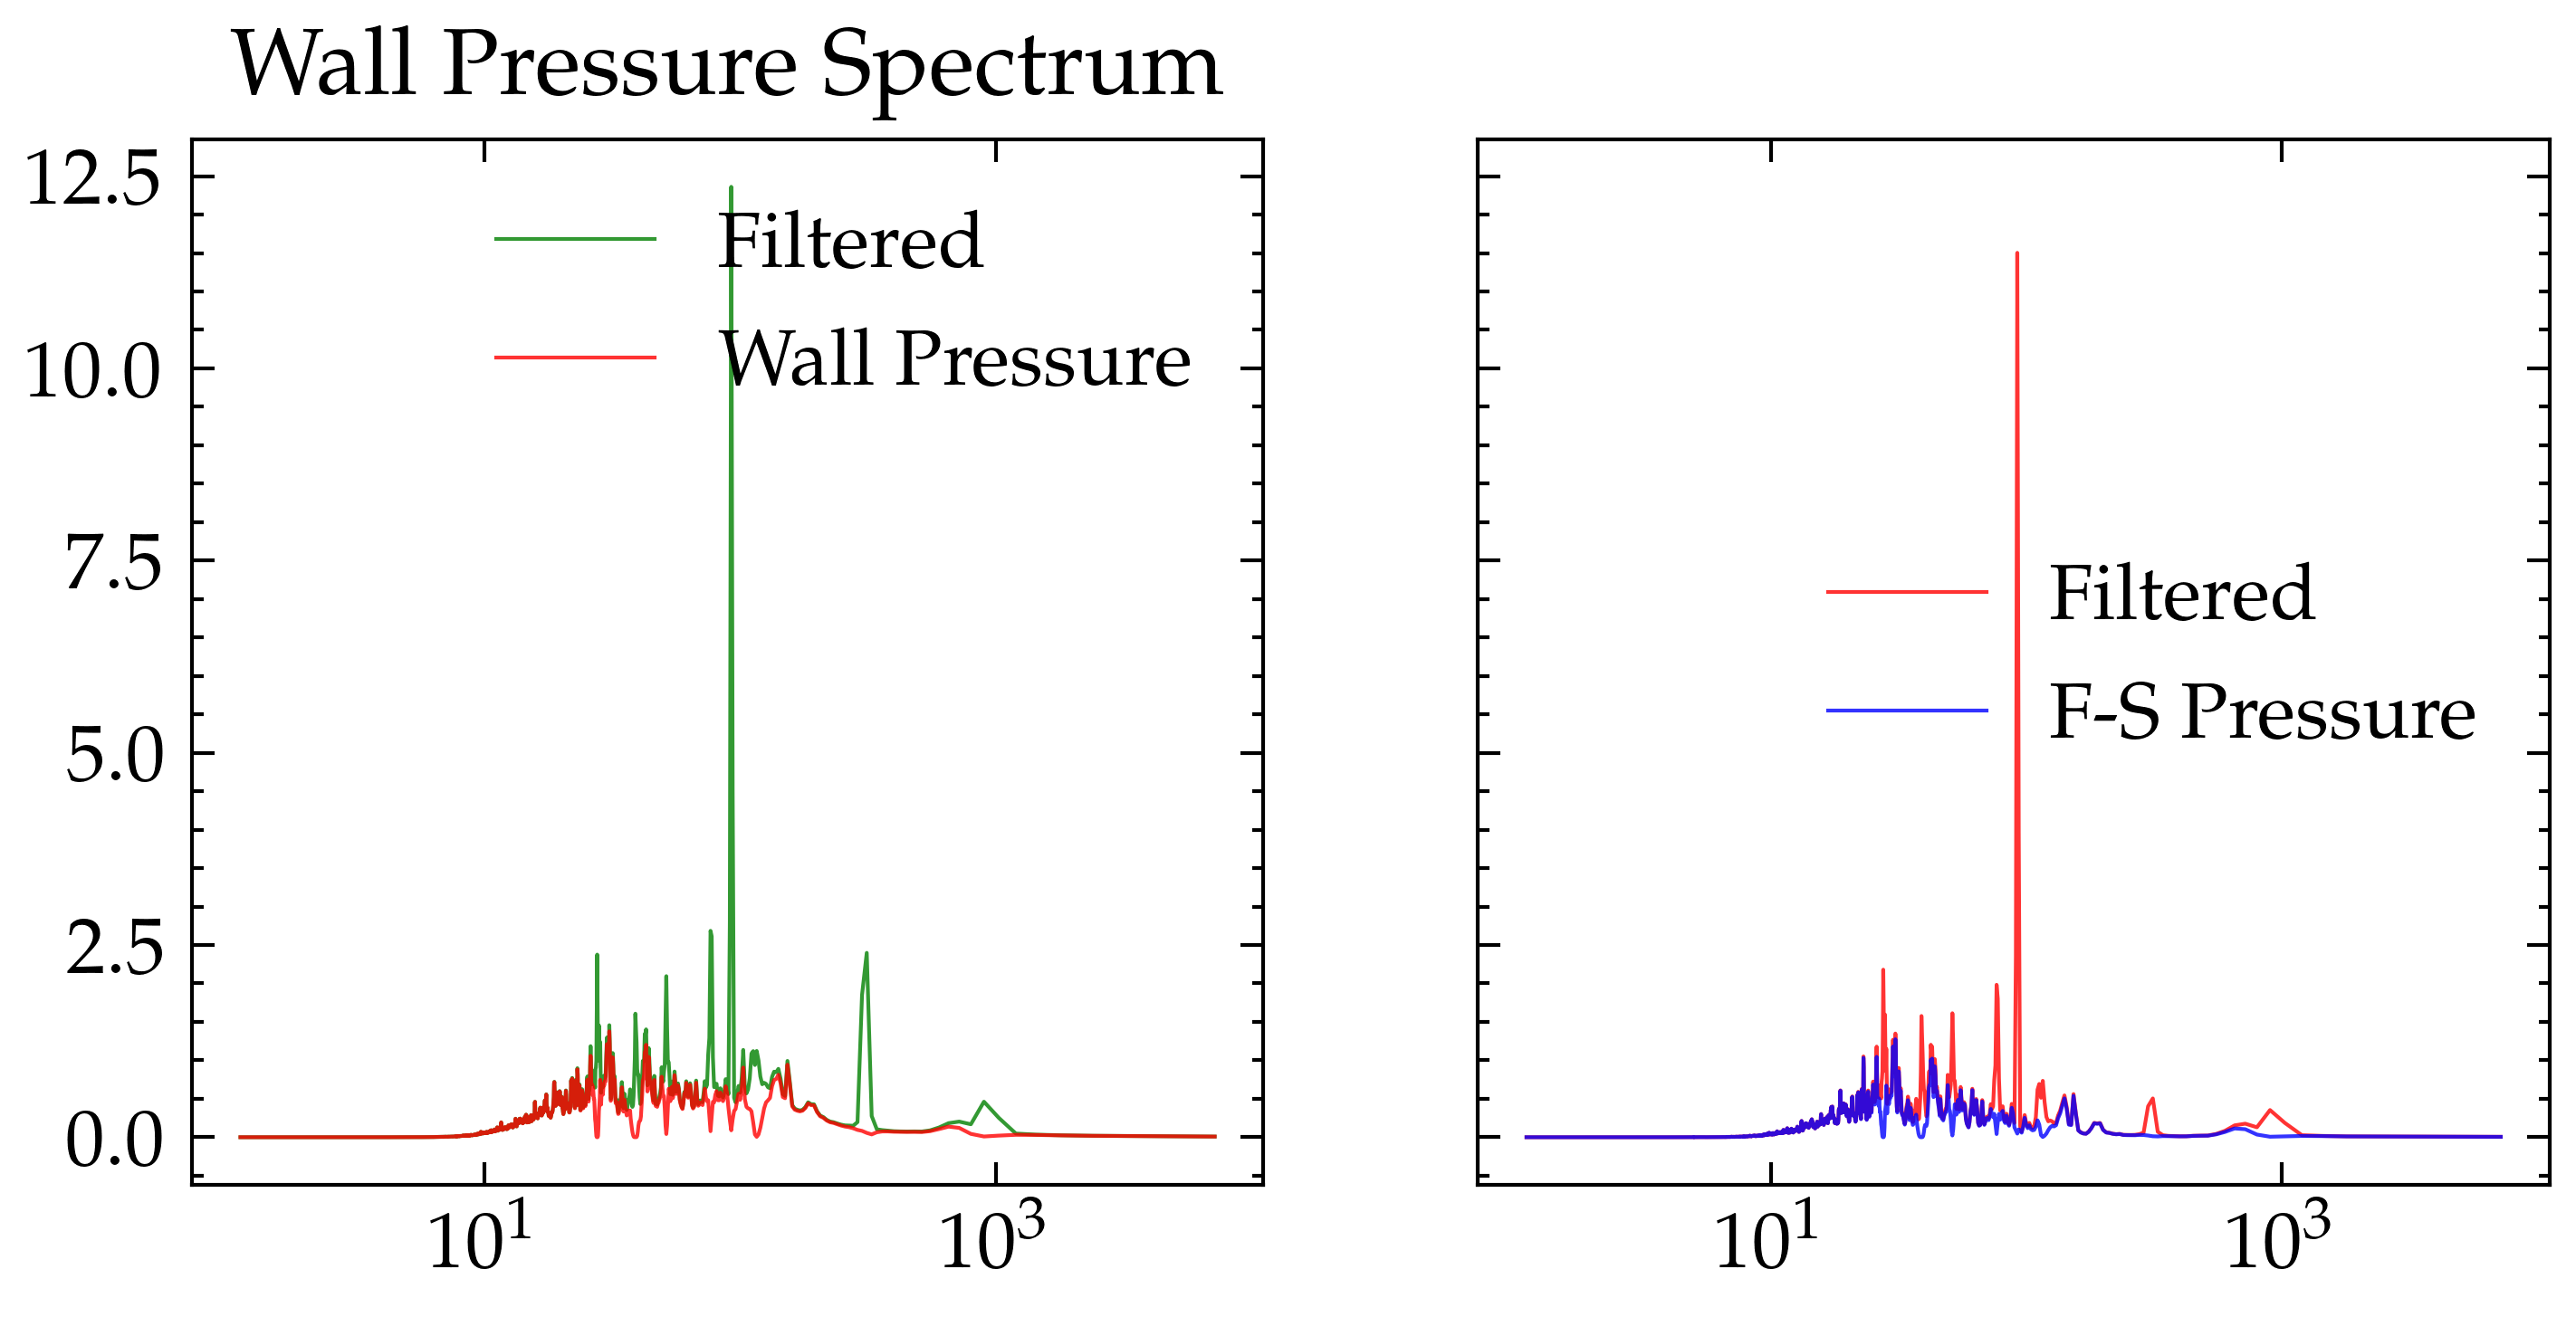
\includegraphics[width=0.7\linewidth]{figures/notched_pressure_spectrum.png}
    \begin{itemize}
            \centering
        \item Filter signal with bandwidth filter in the timeseries
    \end{itemize}

\end{frame}

\begin{frame}{Coherence between wall and free-stream pressure}
    \centering
    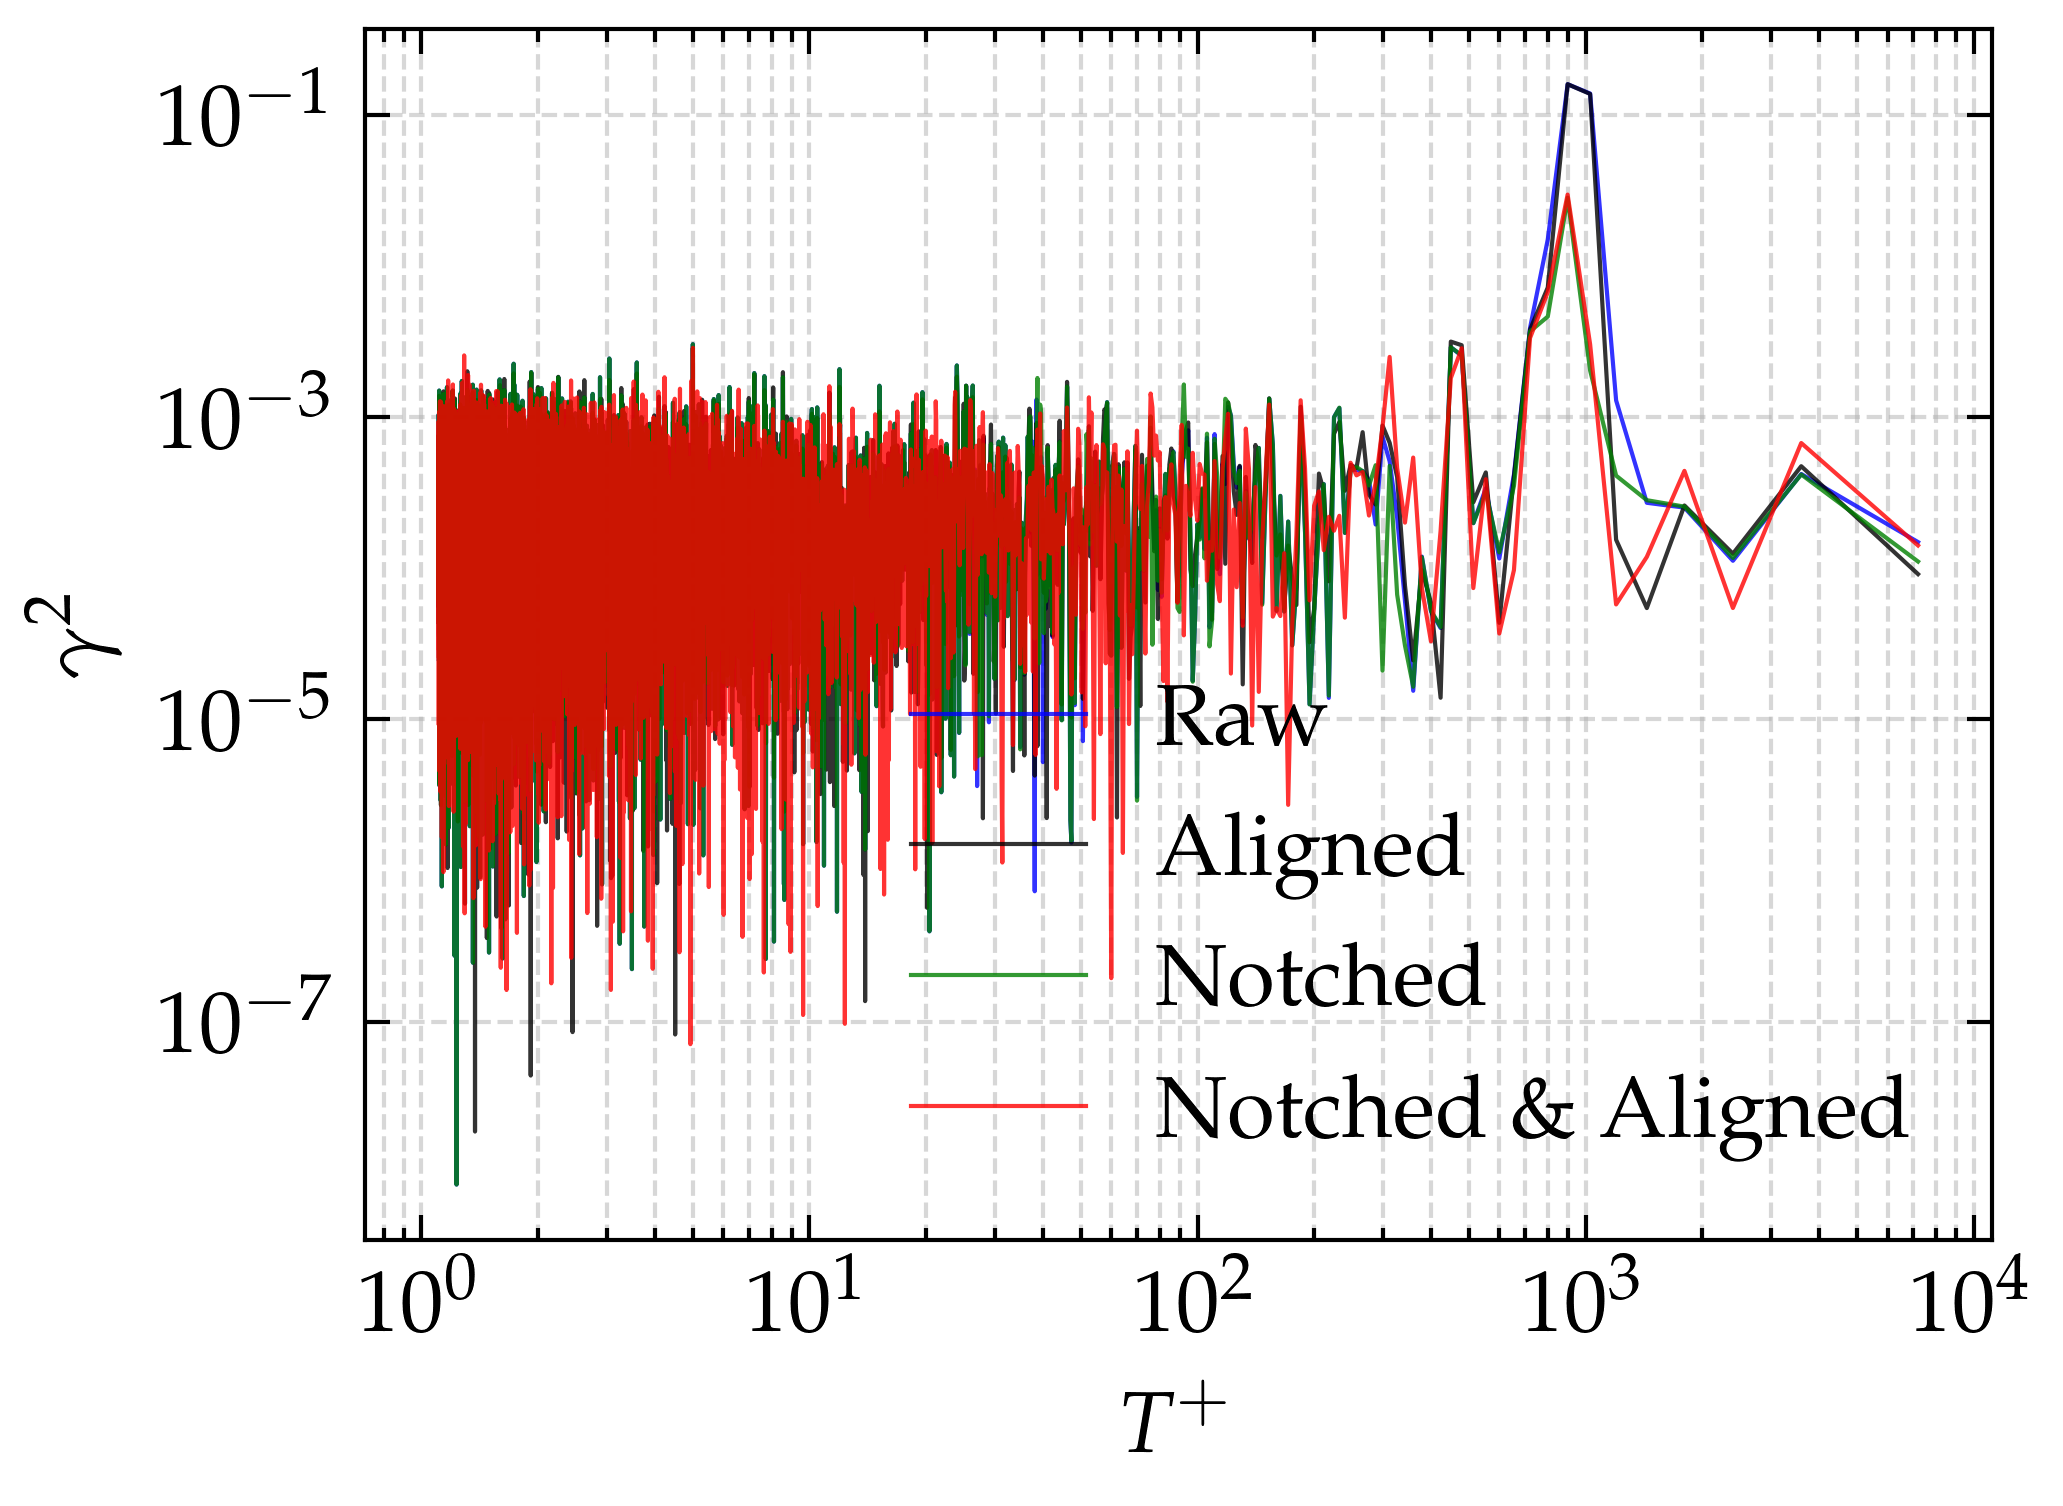
\includegraphics[width=0.5\linewidth]{figures/coherence.png}
    \begin{itemize}
        \centering
        \item Miss-alignment of F-S and Wall mic causes a phase shift
        \item Maximised coherence based on time lag
        \item Still uncorrelated
    \end{itemize}
\end{frame}

\begin{frame}{Transfer function between reference spectra and measurements}
    \centering
    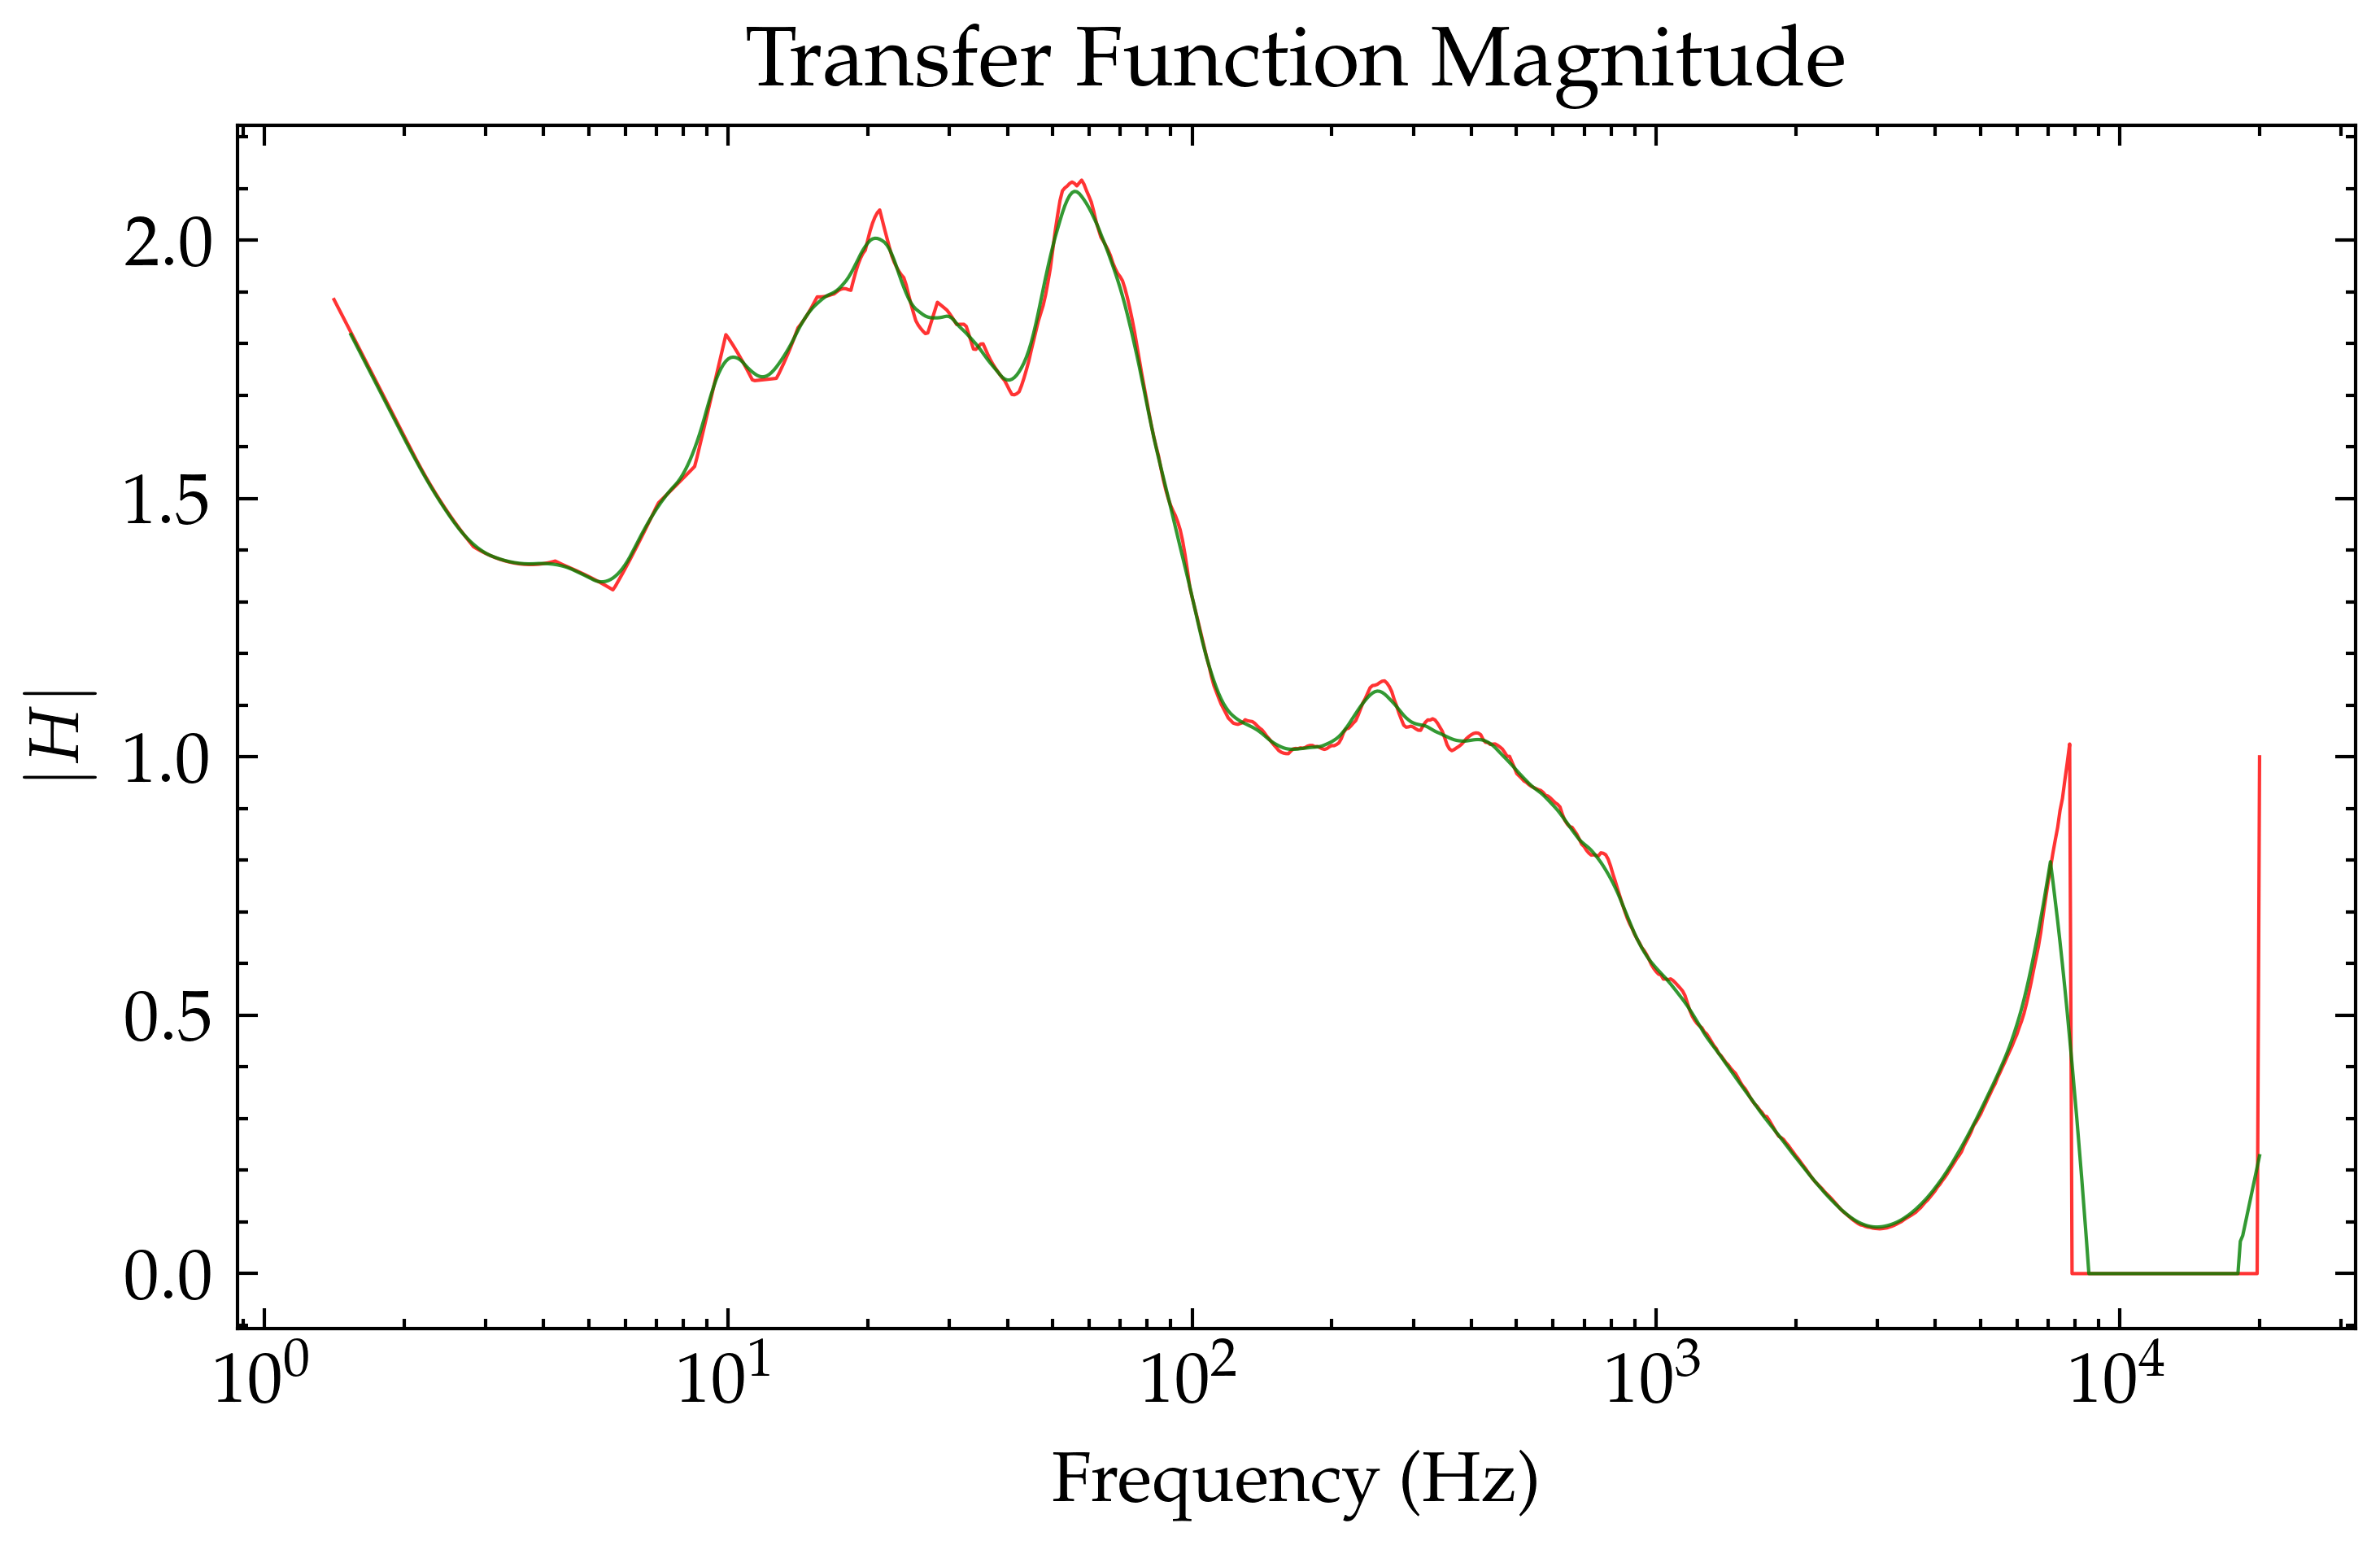
\includegraphics[width=0.7\linewidth]{figures/transfer_function_magnitude.png}
    \begin{itemize}
        \centering
        \item Transfer function between reference spectra and measurements
    \end{itemize}
\end{frame}

\begin{frame}{Corrected signals}
    \centering
    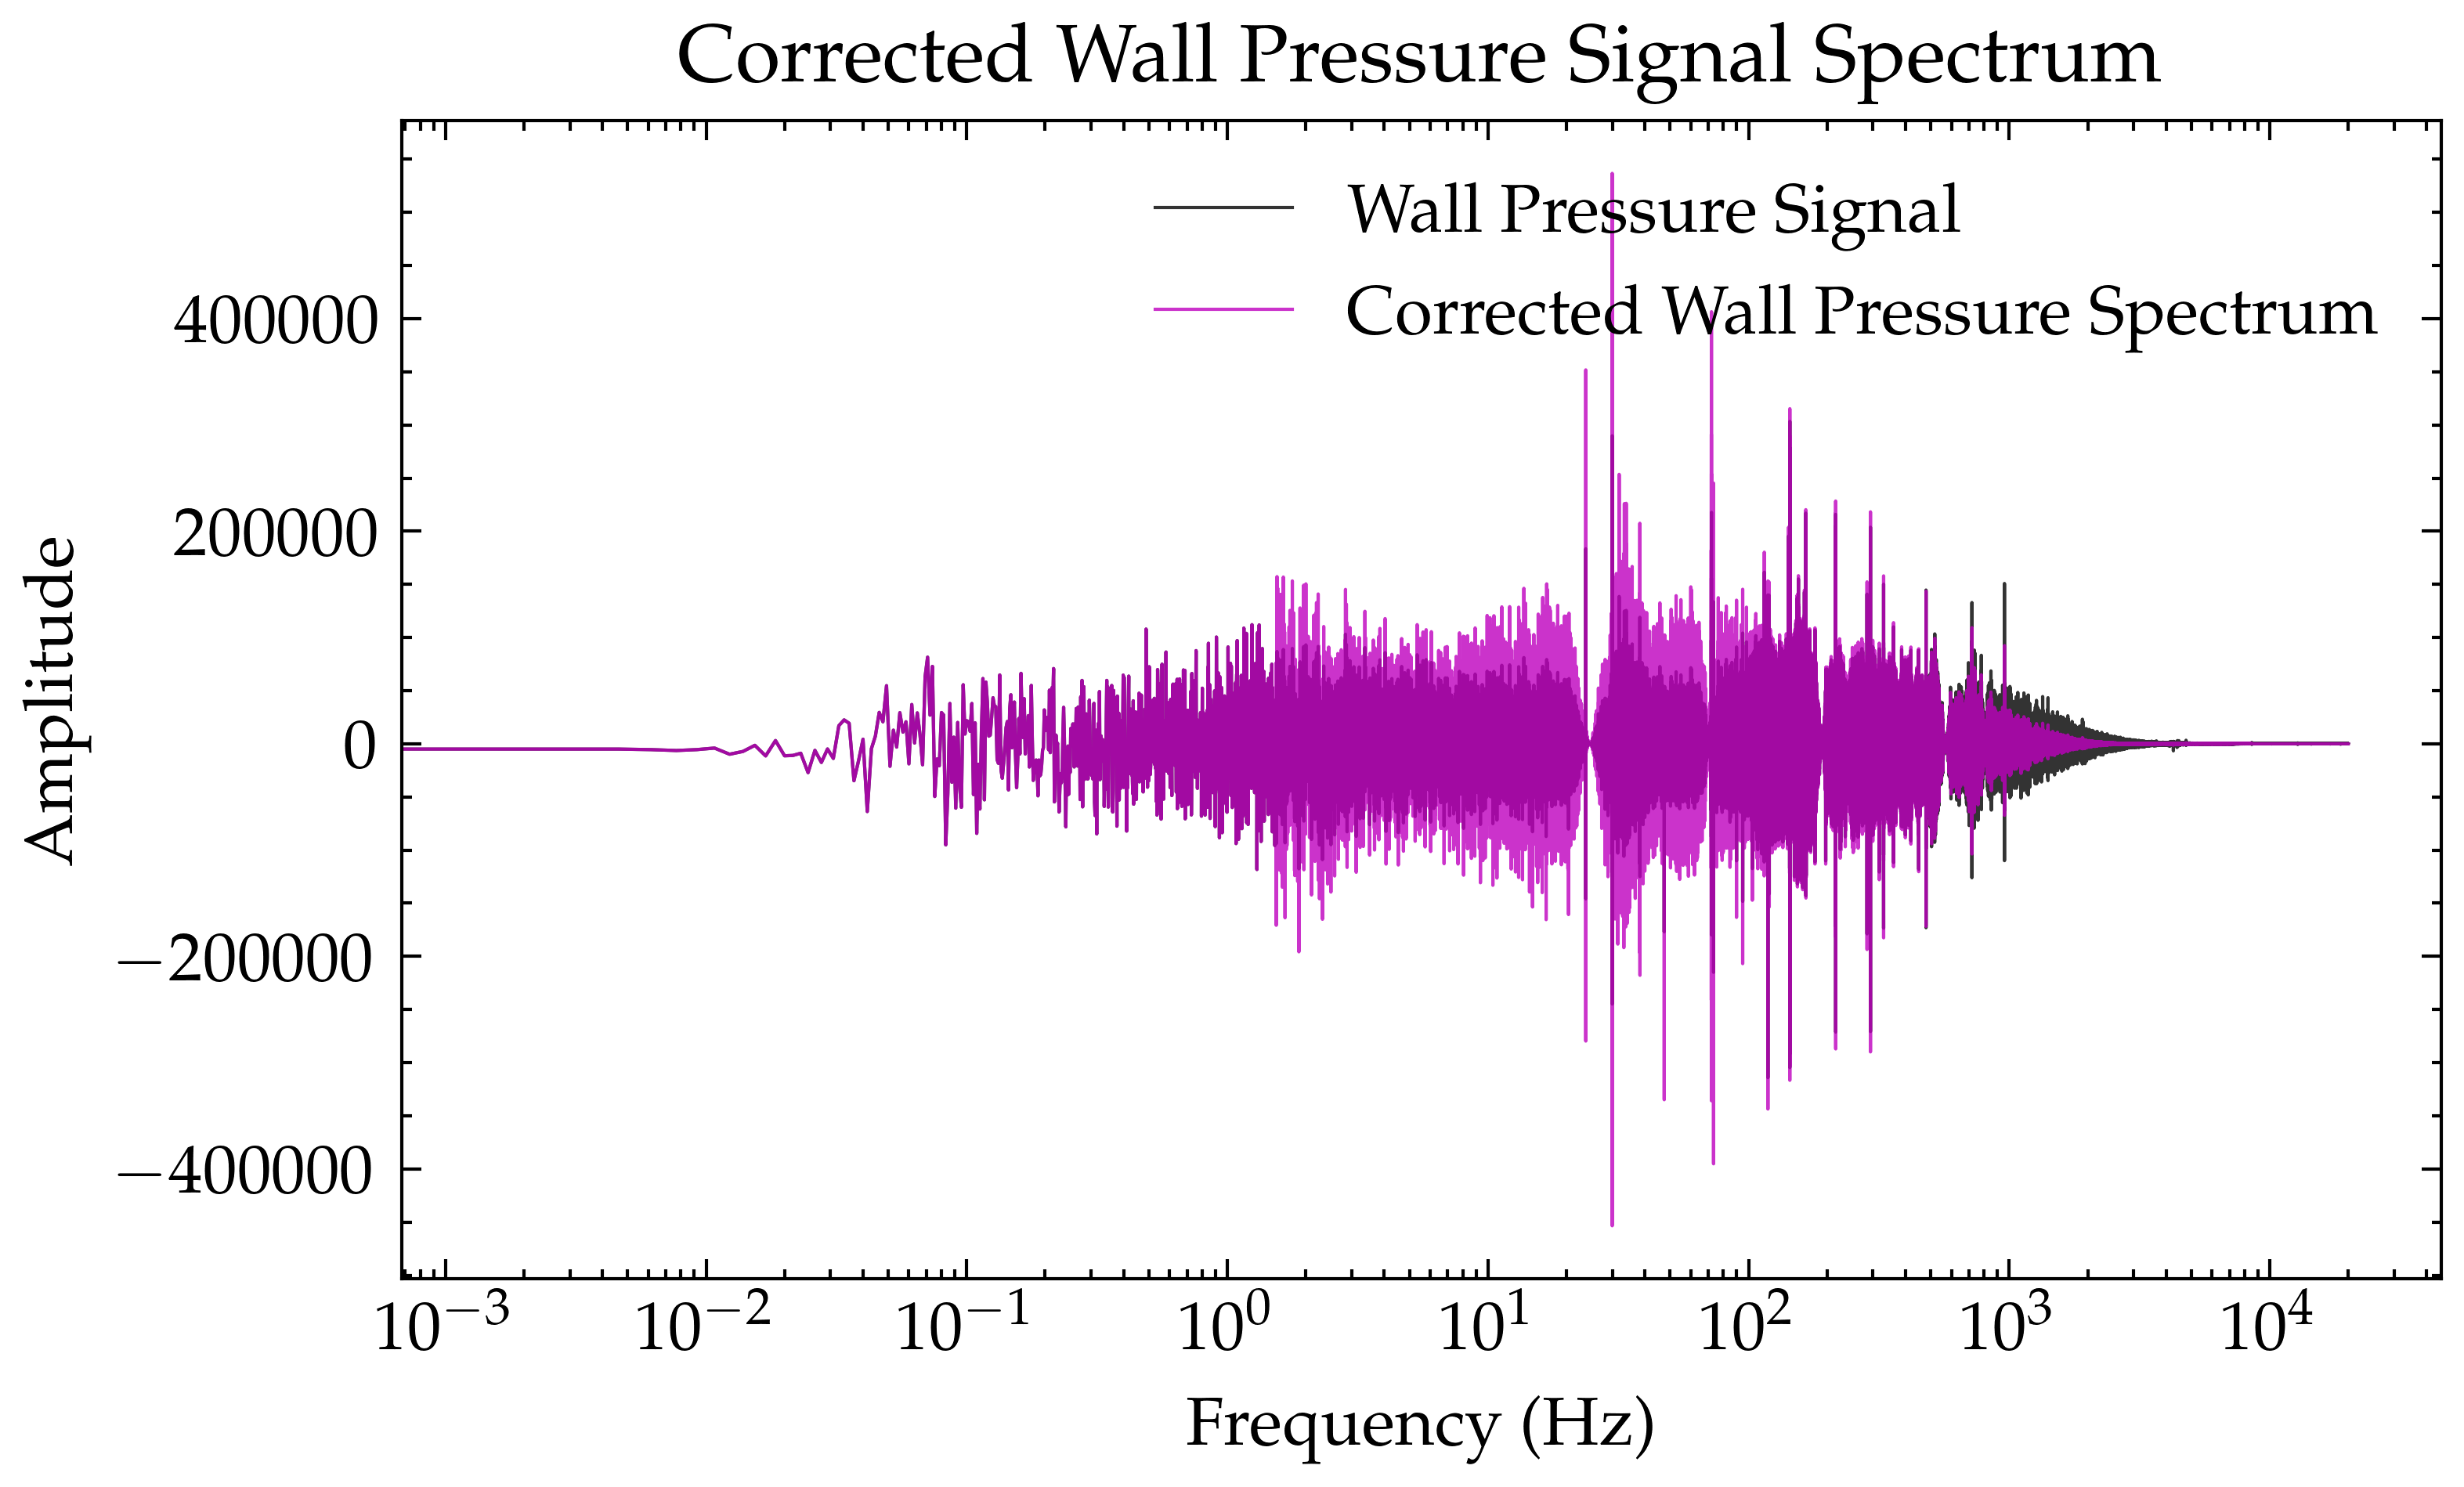
\includegraphics[width=0.7\linewidth]{figures/corrected_wall_pressure_signal_spectrum.png}
    \begin{itemize}
        \centering
        \item Corrected wall pressure signal spectrum
    \end{itemize}
\end{frame}

\begin{frame}{Corrected spectra}
    \centering
    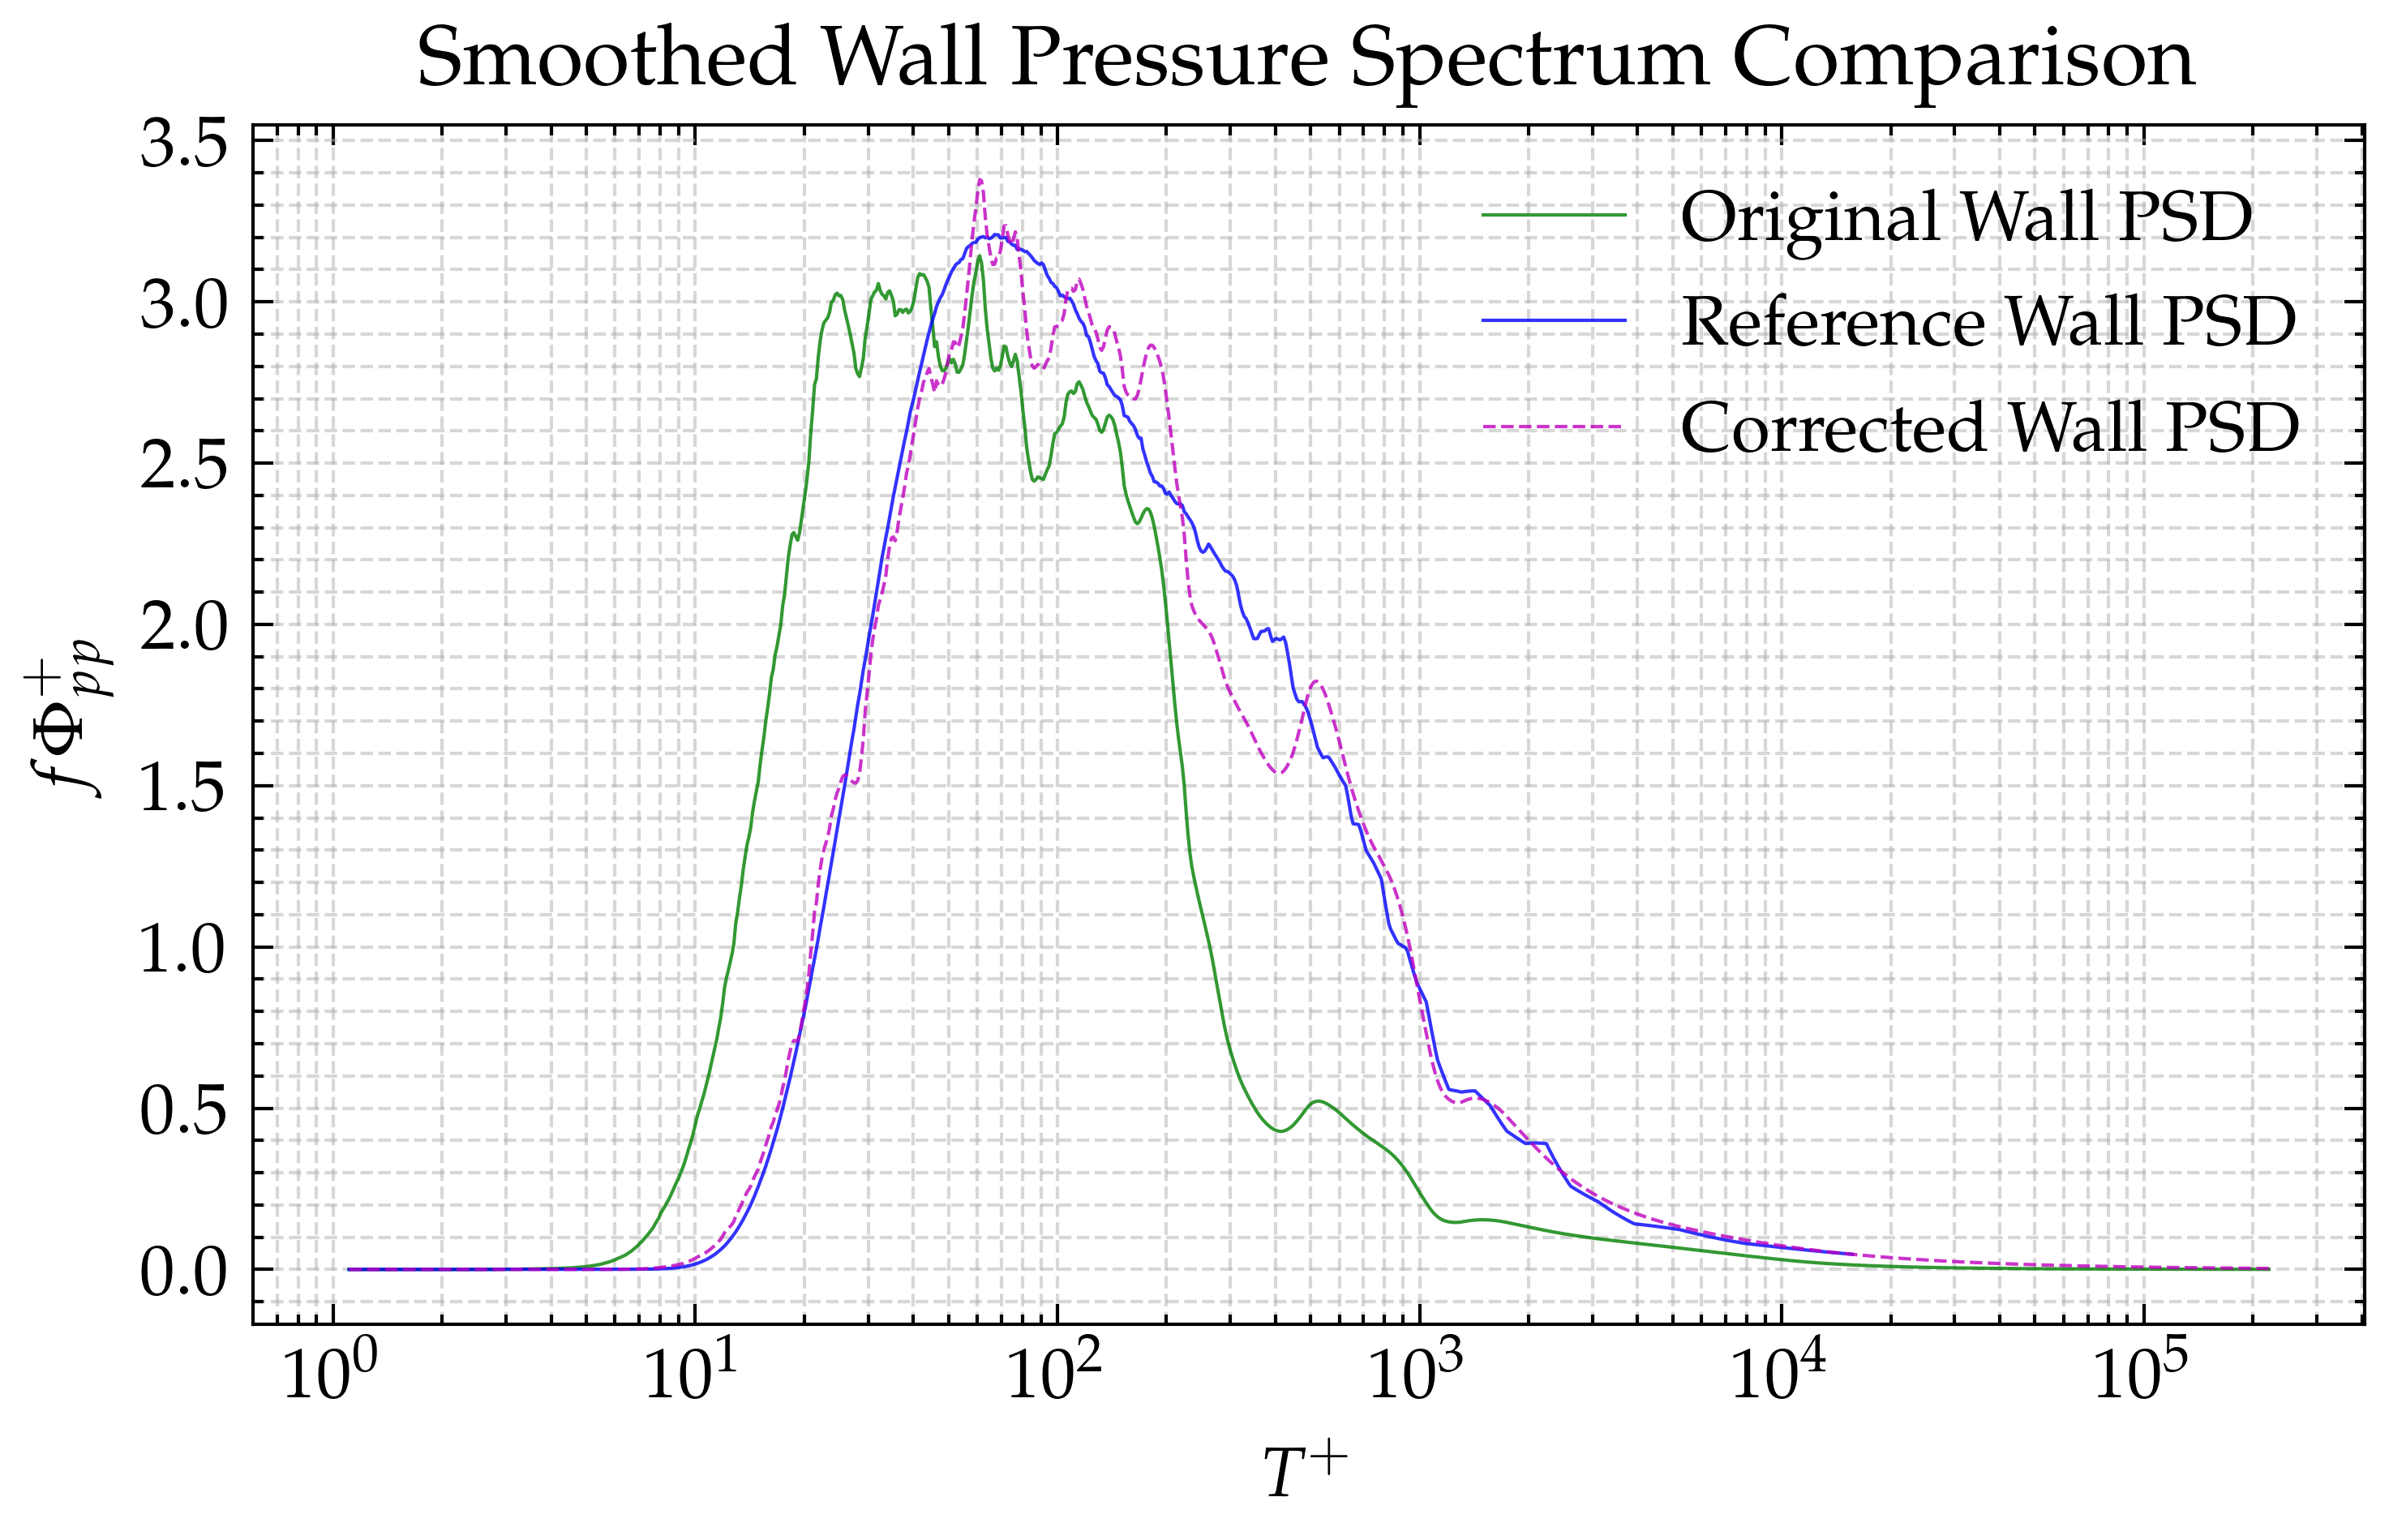
\includegraphics[width=0.7\linewidth]{figures/corrected_wall_pressure_spectrum.png}
\end{frame}

\begin{frame}[noframenumbering,allowframebreaks]
    \frametitle{References}
    \bibliographystyle{jfm}
    \bibliography{refs}
\end{frame}

% \section{Backup}
% \include{sections/greens}

\end{document}
